\begin{figure}[H]
\centering
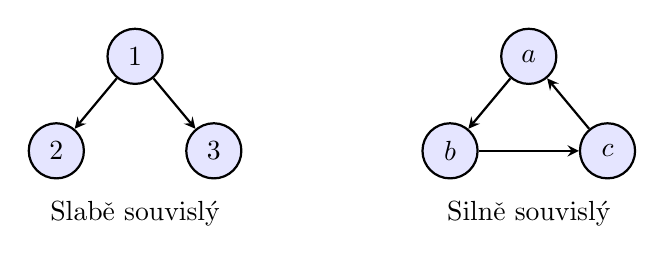
\begin{tikzpicture}[
  vnode/.style={circle, draw, minimum size=7mm, inner sep=0pt, fill=blue!10},
  thick,
  >=stealth
]
  % Slabě souvislý (vlevo)
  \begin{scope}[shift={(-2.5,0)}]
    \node[vnode] (1) at (0, 0.8) {1};
    \node[vnode] (2) at (-1, -0.4) {2};
    \node[vnode] (3) at (1, -0.4) {3};
    \draw[->] (1) -- (2);
    \draw[->] (1) -- (3);
    \node at (0, -1.2) {Slabě souvislý};
  \end{scope}

  % Silně souvislý (vpravo)
  \begin{scope}[shift={(2.5,0)}]
    \node[vnode] (a) at (0, 0.8) {$a$};
    \node[vnode] (b) at (-1, -0.4) {$b$};
    \node[vnode] (c) at (1, -0.4) {$c$};
    \draw[->] (a) -- (b);
    \draw[->] (b) -- (c);
    \draw[->] (c) -- (a);
    \node at (0, -1.2) {Silně souvislý};
  \end{scope}
\end{tikzpicture}
\caption{Ukázka slabě souvislého grafu (z vrcholu 2 se nelze dostat nikam, ale po ignorování šipek je souvislý) a silně souvislého grafu (obsahuje orientovaný cyklus).}
\end{figure}